\documentclass{article}

% if you need to pass options to natbib, use, e.g.:
%     \PassOptionsToPackage{numbers, compress}{natbib}
% before loading neurips_2019

% ready for submission
% \usepackage{neurips_2019}

% to compile a preprint version, e.g., for submission to arXiv, add add the
% [preprint] option:
%     \usepackage[preprint]{neurips_2019}

% to compile a camera-ready version, add the [final] option, e.g.:
%\usepackage[final]{neurips_2019}

% to avoid loading the natbib package, add option nonatbib:
%\usepackage[nonatbib]%{neurips_2019}

\usepackage[utf8]{inputenc} % allow utf-8 input
\usepackage[T1]{fontenc}    % use 8-bit T1 fonts
\usepackage{hyperref}       % hyperlinks
\usepackage{url}            % simple URL typesetting
\usepackage{booktabs}       % professional-quality tables
\usepackage{amsfonts}       % blackboard math symbols
\usepackage{nicefrac}       % compact symbols for 1/2, etc.
\usepackage{microtype}      % microtypography
\usepackage{graphicx,wrapfig,lipsum}
\usepackage[english]{babel}
\usepackage{setspace}
%\usepackage[authoryear]{natbib}
% \usepackage[style=authoryear-ibid,backend=biber]{biblatex}
% \usepackage[numbers]{natbib}
% \addbibresource{Diss_refs.bib}
% \bibliography{Diss_refs.bib}
\usepackage{natbib}
\usepackage{hyperref}
\usepackage{amsmath}
\usepackage{geometry}
\usepackage{enumerate}
%\usepackage{biblatex}
%\bibliography{testcrabbib} % Entries are in the "testcrabbib.bib" file
%\usepackage[square,numbers]{natbib}

% \title{
% \author{}
% \vspace{1pt}
% \normalsize
%   690026937\\
%   \normalsize
%   College of Life and Environmental Science\\
%   \normalsize
%   University of Exeter\\
%   \date{}
%   \hspace{-5mm}
%   \centerline{\rule{1\linewidth}{1.0pt}}
% \small
% University of Exeter\\
% % \hspace*{+55mm}
% \small
% College of Life and Environmental Science\\
% %\end{minipage}
% % \end{}
% \centerline{\rule{1\linewidth}{3.0pt}}
% \vspace{5pt}
% \huge
% Trends in subsurface phytoplankton abundance at the Bermuda Atlantic Time-series Study
% }
% \vspace{10pt}
% \includegraphics[width=8cm, trim=0 0 0 +12cm]{University-of-Exeter-Logo.jpg}
% The \author macro works with any number of authors. There are two commands
% used to separate the names and addresses of multiple authors: \And and \AND.
%
% Using \And between authors leaves it to LaTeX to determine where to break the
% lines. Using \AND forces a line break at that point. So, if LaTeX puts 3 of 4
% authors names on the first line, and the last on the second line, try using
% \AND instead of \And before the third author name.



  % examples of more authors
  % \And
  % Coauthor \\
  % Affiliation \\
  % \texttt{email} \\
  % \AND
  % Coauthor \\
  % Affiliation \\
  % Address \\
  % \texttt{email} \\
% }

\begin{document}


%\noindent\begin{minipage}{0.1\textwidth}% adapt widths of minipages to your needs
%\includegraphics[width=3cm, trim=0 0 0 0]{University-of-Exeter-Logo.jpg}
%\end{minipage}%
%\hfill%
%\begin{minipage}{1\textwidth}\raggedright
%\hspace*{+52mm}
%University of Exeter\\
%\hspace*{+55mm}
%College of Life and Environmental Science\\
%\end{minipage}
% \end{}

\title{
\huge
Trends in subsurface phytoplankton biomass at the Bermuda Atlantic Time-series Study \\
\normalsize
\vspace{0.8cm}
690026937 \\
\vspace{0.5cm}
Supervised by Dr Bob Brewin \\
\begin{center}
\includegraphics[width=10cm, trim=+0cm 0 0 -1cm]{University-of-Exeter-Logo.jpg}
\end{center}
\vspace{}

}
\maketitle
\begin{center}
  Word count: 4958\\
  \vspace{0.5cm}
  Number of figures, tables and text boxes: 3\\
  \vspace{1cm}
  \small
  I declare that this dissertation is entirely my own work and no part of it has been submitted for a degree or other qualification in this or another institution and give permission for a copy to be held by my supervisor and distributed at their discretion
\end{center}

\newpage
\tableofcontents
\newpage
\setstretch{1.5}
\section{Abstract}
Phytoplankton are involved in important global marine biogeochemical cycles. Due to the progressive impacts of climate change on phytoplankton, it is therefore essential to understand how they are changing globally. However, common phytoplankton monitoring techniques exclude or cannot distinguish the rich community of phytoplankton that occur below the surface layer. Here, by applying a recently developed model to vertical longitudinal data from an open ocean site, long term trends in surface and subsurface communities are investigated separately for the first time. It is shown that, using Chlorophyll-a as a proxy for phytoplankton biomass, total biomass at the site was maintained while the subsurface community increased in biomass and the surface community decreased in biomass over 28 years. These results highlight the importance of monitoring subsurface phytoplankton and are contrary to predictions of global phytoplankton decline, with potential ramifications for similar ocean regions around the world.

\section{Introduction}
Phytoplankton are photosynthetic microorganisms that are present in the photic zone across the world’s oceans. Communities of phytoplankton are a groups of phytoplankton species that inhabit the same area at the same time. In consequence of their high abundance and productivity, contributing to around half of global primary production \citep{field_primary_1998}, phytoplankton influence the biogeochemical cycles of the Earth. They play a pivotal role in the carbon cycle, with the production of organic carbon through photosynthesis and its sequestration in the deep ocean \citep{street_iron_2005}; future changes to phytoplankton communities are therefore integral to predicting future atmospheric carbon dioxide concentrations \citep{passow_u_biological_2012}. Phytoplankton also form the bedrock of the marine ecosystem, with any variations in a community having knock-on effects for marine organisms from all trophic levels including humans \citep{vargas_phytoplankton_2006,danielsdottir_phytoplankton_2007}. Through the impacts of anthropogenic climate change such as ocean acidification and ocean warming on phytoplankton, we have already observed subsequent changes to the carbon cycle \citep{herrmann_impact_2014} and marine ecosystems \citep{frederiksen_plankton_2006}, highlighting the need to increase understanding of how phytoplankton communities are changing. \\ \\
\noindent
Phytoplankton communities have the potential to change in response to climate change in many ways, disrupting biogeochemical cycles. One such way is the physiological changes in individual plankton. Coccolithophores are a major group of phytoplankton that are uniquely involved in marine calcium cycles, due to their calcium carbonate exoskeletons, and contribute significantly to ocean carbon sequestration \citep{arundhathy_coccolithophores_2021}. Due to physiological changes in their exoskeletons in response to more acidic environments, some common coccolithophore species have been demonstrated to reduce calcification and photosynthetic rates in response to ocean acidification, which could reduce their prevalence \citep{meyer_reviews_2015}. This illustrates how escalating factors like ocean acidification, which disproportionally affect the physiology of certain species (such as coccolithophores), could alter a phytoplankton community’s involvement in nutrient cycles \citep{marinov_response_2010,mcmahon_millennial-scale_2015}. Due to specialisation of predator species, this involvement could cause fundamental ecosystem changes that propagate up to the higher trophic levels \citep{frederiksen_plankton_2006}.\\ \\
\noindent
Another way in which phytoplankton communities may change is through their phenology, via the timing of seasonal blooms. Spring phytoplankton blooms are relatively short events consisting of mass increases in phytoplankton populations that can amount to one-third of annual production and over one-half of annual organic matter that sinks to the seafloor \citep{townsend_causes_1994}. The timing of these historically consistent blooms is affected by changes in wind mixing, the mixed layer depth (MLD) and ocean temperatures - factors that are influenced by climate change \citep{townsend_causes_1994,gittings_impacts_2018,sommer_climate_2008}. Furthermore, variation in the timings of these blooms, resulting in mismatches between phytoplankton blooms and marine fish spawning events, has been linked to lowered recruitment rates of marine fish \citep{asch_climate_2019}. This shows the role phytoplankton phenology plays in the impacts of climate change on marine ecosystems, highlighting how the monitoring of phytoplankton communities is important in assessing the effects of climate change on marine ecosystems and fish stocks.\\ \\
\noindent
Surface observations of phytoplankton over the last century have revealed declines of biomass in eight out of ten of the world’s ocean regions, with the global rate of phytoplankton decline being estimated at $\sim$1\% per annum \citep{boyce_global_2010}. Furthermore, in this study these trends were linked to increases in sea surface temperature (SST), which have globally been linked to anthropogenic climate forcing \citep{gittings_impacts_2018,boyce_global_2010,deser_twentieth_2010}. This demonstrates how long-term declines in surface phytoplankton biomass are tied to the developing impacts of climate change through SST. Long-term changes in phytoplankton biomass and productivity have been linked to regime shifts in phytoplankton communities \citep{mcquatters-gollop_long-term_2007}. As regime shifts in phytoplankton community structures have been shown to significantly alter that community’s role in nutrient cycling and ecosystem function \citep{mcmahon_millennial-scale_2015,brothers_regime_2013}, this signposts how important the understanding and monitoring of trends in phytoplankton biomass is for assessing the impacts of climate change on global biogeochemical cycles.\\ \\
\noindent
As mentioned, shallowing of the MLD contributes to the development of phytoplankton blooms, as it increases light availability, promoting phytoplankton growth \citep{townsend_causes_1994,gittings_impacts_2018}. However, an understudied community of phytoplankton resides below this mixed layer in the euphotic zone in over $70\%$ of the world’s waters, where the water column is permanently or seasonally stratified \citep{cullen_subsurface_2015,cullen_deep_1982}. This subsurface phytoplankton community holds a significant proportion of total phytoplankton biomass in the water column, with blooms that occur for longer more sustained periods of time than those in the surface community \citep{ross_blooms_2017}. These hard-to-measure subsurface phytoplankton blooms have also been hypothesised to be the drivers of summer primary production in temperate marine systems \citep{richardson_subsurface_2000}. These findings display the relevance of subsurface phytoplankton communities when discussing the importance and impacts of changes in global phytoplankton. \\ \\
\noindent
Though studies on trends in global surface phytoplankton display clear evidence of declining biomass \citep{boyce_global_2010}, research analysing long-term time-series data on phytoplankton in the entire water column (including the subsurface community) has shown that total phytoplankton biomass is both increasing and decreasing in many regions \citep{boyce_dg_patterns_2015}. Most published evidence suggests that coastal regions tend to see increases in phytoplankton biomass because of increases in terrestrial nutrient runoff. In contrast, nutrient deficient (oligotrophic) open ocean regions tend to see decreases in phytoplankton biomass as a result of increased SSTs increasing water column stratification, thereby reducing nutrient flux to the surface from deeper waters \citep{boyce_dg_patterns_2015,dalelio_machine_2020,schmittner_decline_2005}. It should be noted, however, that not all sites follow this trend; at one long-term oligotrophic ocean study site (the Hawaiian Ocean Time-series) chlorophyll-a (used as a proxy for biomass) has been shown to be increasing \citep{saba_challenges_2010}.\\ \\
\noindent
With depth, subsurface phytoplankton community chlorophyll production typically culminates to a deep- or subsurface chlorophyll maximum (DCM or SCM), a region where chlorophyll-a (Chl-a) produced by phytoplankton peaks in the water column. In some areas, the SCM can account for over $70\%$ of total Chl-a in the water column \citep{zhuang_phytoplankton_2020}; deep chlorophyll maxima have also been hypothesised as the site of diatoms production. Diatoms are a large group of silica-based phytoplankton that are an important part of marine ecosystems, being marked as a keystone species in nutrient cycling \citep{medlin_why_2002}. This signposts the ecological importance of vertical phytoplankton community structure and brings to attention the idea that monitoring changes in the subsurface community could provide insight into ocean primary production and, by extension, changes in geochemical cycles and ecosystems \citep{boyce_global_2010,ross_blooms_2017}.\\ \\
\noindent
However, subsurface phytoplankton communities remain relatively understudied, largely due to the cost and difficulty of monitoring \citep{hogle_pervasive_2018}. Monitoring of phytoplankton typically utilises Chl-a concentration measurements as a proxy for biomass. Due to physiological variations in intracellular Chl-a in response to conditions such as light and temperature \citep{behrenfeld_beam_2006,geider_dynamic_1996}, Chl-a concentration measurements vary independently from phytoplankton biomass along the vertical distribution. This is thought to result from shifts in photoacclimation as light attenuates with depth \citep{cullen_subsurface_2015,fennel_subsurface_2003}. The use of Chl-a concentration measurements as a proxy of phytoplankton is further complicated by the measurements varying with underwater photosynthetically active radiation and nutrient concentrations \citep{alvarez-fernandez_chlorophyll_2014}. Despite this Chl-a concentration has remained the most widely used measure of phytoplankton biomass in ecological studies as it is relatively easy to measure \citep{boyce_global_2010}.\\ \\
\noindent
Satellite radiometry datasets are most commonly used in studies on global phytoplankton biomass as no other form of monitoring provides the high frequency, long-term and wide surface-level coverage that satellite remote sensing provides \citep{siegel_century_2010}. However, satellite spectroradiometers can only penetrate the surface layer of the water column, leaving most of the subsurface phytoplankton community unaccounted for in these datasets \citep{cornec_deep_2021}. For subsurface observations, ocean robotic platforms such as biogeochemical Argo floats can be used \citep{su_subsurface_2021}. However, data from these platforms are both relatively recent \citep{xing_toward_2018} and short in length due to the short lifespans of these floats ($\sim$5 years) \citep{williams_calculating_2017}. Ship-based surveys at ocean stations provide datasets with very limited spatial coverage. Nevertheless, these datasets can provide long-term, frequent, and high-quality observations on phytoplankton biomass below the surface layer, making them suitable for observing long-term subsurface trends.\\ \\
\noindent
New advances in phytoplankton community modelling now allow for the partitioning of phytoplankton biomass into surface and subsurface communities in chlorophyll-depth profiles \citep{lange_phytoplankton_2018,brewin_conceptual_2022}. This provides the opportunity to specifically study the elusive subsurface community in chlorophyll-depth profiles like those found in Argo float and boat survey datasets. \\ \\
\noindent
Here, local longitudinal oceanographic data is analysed using a novel partitioning model \citep{brewin_conceptual_2022} to investigate the surface and subsurface phytoplankton communities separately. This study aimed to find any long-term trends in the biomass of the subsurface phytoplankton community. 
\noindent
\section{Method}
All data processing, analysis and visualisation were completed in Python 3.9.7 \citep{van_rossum_python_2009}.
\noindent
\subsection{Overview}
\subsubsection{Oceanographic Data Selection}
Data from the Bermuda Atlantic Time-Series Study (BATS) was selected for use in this project. This decision was made based on: (i) the length of the dataset, as regular data collection started in 1989 making the data sufficient for finding long-term trends; (ii) the presence of \textit{in situ} and \textit{in vitro} datasets, as the more accurate \textit{in vitro} data could be used to calibrate the high frequency \textit{in situ} data \citep{wolfe_experimental_2006}; and (iii) the location and conditions of the study site, as the similarity of this site to other large oligotrophic subtropical ocean gyre regions would make any findings from this study have implications for those regions of the ocean \citep{alkire_using_2013}.
\noindent
\subsubsection{Data Collection}
The BATS site is located in subtropical, open oligotrophic water off the coast of Bermuda at the Sargasso Sea, North Atlantic Ocean (31°40’N 64°10’W). Further details on the structure of methods used on BATS cruises are available in published form \citep{knap_bats_1997,steinberg_overview_2001,johnson_chapter_nodate}. \\ \\
\noindent
The BATS CTD and Bottle datasets are free-to-access from https://simonscmap.com/catalog/dataset
s/BATS\%20CTD \& https://simonscmap.com/catalog/datasets/BATS\%20Pigments respectively.
The datasets were downloaded for this project using simonscmap.com, so as to limit the download size of each by selecting only the top 1000m of data \citep{steinberg_overview_2001}.

\subsubsection{CTD Dataset}
CTD (conductivity/temperature/depth) readings were taken from November 1988 through December 2016, totalling 1750041 observations over 4659 vertical profiles, measuring Temperature (°C), Fluorescence (relative fluorescence units) which had been processed to Chl-a concentration ($\mu g$ $l ^{-1}$) and Pressure (decibar) which had been converted to Depth (m). Two periods without significant fluorescence data occur between 1992 and 1995 and in 2007. This dataset as well as further details of the methods used in its compilation are available in published form \citep{knap_bats_1997,johnson_chapter_nodate-1}. \\ \\
\noindent
This dataset posed two issues in its original form. \textit{In situ} fluorescence readings from fluorometers progressively skew without regular recalibration when used. Another common issue with \textit{in situ} fluorometer readings is the non-photochemical quenching (NPQ) distortion, where phytoplankton biomass is underestimated because of the high light levels found near the surface causing a reduction in phytoplankton pigmentation in the mixed layer \citep{holte_new_2009}. In this study, an NPQ correction was used to combat this underestimation of surface phytoplankton \citep{schmechtig_bio-argo_2018}, while the fluorescence readings were calibrated to the more accurate BATS \textit{in vitro} Bottle dataset to correct skewed fluorometer readings. Details of the methodology of these corrections can be found below in \textit{3.2.2 NPQ Correction} and \textit{3.2.3 Fluorescence Calibration}.
\subsubsection{Bottle Dataset}
Water samples were collected in vertical profiles from November 1988 through December 2016. Sample analysis was conducted at the Bermuda Biological Station for Research. Water samples were filtered for chlorophyll-a and two techniques were used for analysis, first using high-performance liquid chromatography (HPLC, $ng$ $l ^{-1}$) and secondly by using \textit{in vitro} fluorometry (Turner, $\mu g$ $l ^{-1}$). These measurements were deemed as more accurate readings of Chl-a concentration than those in the CTD dataset due to the absence of errors common with \textit{in situ} fluorometer readings \citep{gregor_freshwater_2004}. The dataset was of a lower frequency than the CTD dataset, totalling 4896 observations over 365 vertical ocean profiles. These data as well as details of the methods used are available in published form \citep{knap_bats_1997,rathbun_chapter_nodate}. 
\subsection{Data Processing}
Before the data could be analysed, it was compiled into a workable format as detailed below.
\subsubsection{Dataset Cleaning}
First, the .csv files of each dataset were loaded into Python in a 'dataframe' format, where observations with missing readings were removed. In the CTD dataset, this removal applied to rows with absent temperature or fluorescence readings. In the Bottle dataset, this removal applied to rows with both absent Turner Chl-a and HPLC Chl-a readings.\\ \\
\noindent
For the Bottle dataset, both Turner and HPLC Chl-a measurements were available. These measurements were in concordance (mean difference $=$ 0.0125 $\mu g$ $l ^{-1}$) so were combined into a single variable ($\mu g$ $l ^{-1}$) for greater coverage of the time-series. If both measurements were available for a single observation, the mean average was calculated and used in the combined variable.\\ \\
\noindent
Both datasets were subsequently sorted by time and depth to order each vertical profile in the study chronologically. 
\subsubsection{NPQ Correction}
To address non-photochemical quenching distortions present in fluorescence readings in the CTD dataset, a simplified adaptation of the correction developed by \cite{xing_improved_2018} was used. For this correction, the mixed layer depth (MLD) of each profile was required. An algorithm developed by \cite{holte_new_2009} was used to calculate the MLD for each vertical profile, using the temperature and depth data in that profile. Then the maximum fluorescence value in the mixed layer was used to replace all other fluorescence readings above the MLD in each profile.
\subsubsection{Fluorescence Calibration}
To address inaccuracies in the \textit{in situ} fluorometer readings taken during the BATS, CTD fluorometer readings were empirically calibrated to the more accurate Chl-a concentration readings from the Bottle dataset \citep{wolfe_experimental_2006}. Each Bottle Chl-a concentration was divided by its corresponding CTD fluorescence reading, that was taken at the same time and within at least 3m of depth, to find the relative difference. The median average relative difference of every Bottle dataset Chl-a concentration profile was then calculated and compiled into a time-series where a cubic polynomial fit was applied. This modelled the correction as a function of time, allowing correction predictions to be made for CTD profiles without corresponding Bottle data. Finally, all fluorescence readings in each profile in the CTD dataset were calibrated by being multiplied by the value of the average relative difference polynomial fit at the  time the profile was taken.
\subsubsection{Partitioning of Surface and Subsurface Communities}
Using the model developed by \cite{brewin_conceptual_2022} Chl-a concentrations within each profile of the final dataset were partitioned into surface and subsurface phytoplankton communities. The model produced three outputs for each profile: (i) a model fit of total Chl-a (the sum of the surface and subsurface community models); (ii) a model fit of surface community Chl-a, based on a sigmoid function; and (iii) a model fit of subsurface community Chl-a, based on a Gaussian function. \\ \\
\noindent
Each of the model outputs was compiled and ordered into a separate time-series.\\ \\
\noindent
Further details of the modelling code along with examples of it working can be found on a free-to-access GitHub page (https://github.com/rjbrewin/Two-community-phyto-model) while a more detailed explanation of its methodology and function are available \citep{brewin_conceptual_2022}. 
\subsubsection{Integration}
For each model time-series and the calibrated fluorescence data, depth-integrated Chl-a concentration was calculated for each profile using trapezial integration \citep{saba_challenges_2010}. Integration was carried out on each profile from the surface to 1.5x the euphotic depth ($Z_p$). This was in line with reasoning from similar studies on Chl-a modelling and attempts to account for phytoplankton biomass often found below the $Z_p$ \citep{saba_challenges_2010,brewin_modelling_2017,uitz_vertical_2006}. The $Z_p$ was calculated for each profile using the equation from \cite{morel_examining_2007} shown below, where $X$ is the average Chl-a concentration in the mixed layer.\\ \\
% \begingroup
% \Large
% \begin{gather*}
% \begin{equation*}
\begin{center}
    \scalebox{1.6}{$Z_p = 10^{(1.524 - 0.436 * X - 0.0145 * X^{2} + 0.0186 * X^{3})}$}
\end{center}
% \end{equation*}
% \end{gather*}
% \endgroup
\noindent
\\ Compilation of this data into time-series produced the final datasets that would be analysed. These consisted of integrated Chl-a profiles of the raw data and the total model, as well as the modelled surface, and subsurface communities at the Bermuda Atlantic Time-series Study over 28 years.
\subsection{Data Analysis}
For analysis of the data, a linear regression analysis was applied to each model and the original data to find trends in biomass of the total and the two phytoplankton communities at the BATS \citep{angelini_regression_2019}. Only the top 250m of data were investigated as phytoplankton rarely grow below this range \citep{cullen_subsurface_2015}.
\renewcommand{\floatpagefraction}{.88}%66
% \newpage
\section{Results}
\subsection{CTD Dataset Correction and Calibration}
% \setlength{\textwidth}{500pt}

Over all the profiles in the cleaned CTD data (n $=$ 1624724), down to 1000m, the average temperature was 16.7106°C ($Q1 = 18.6313$°C, $Q3 = 15.7606$°C) (Figure 1a).
\begin{figure}[ht!]
\begin{center}
      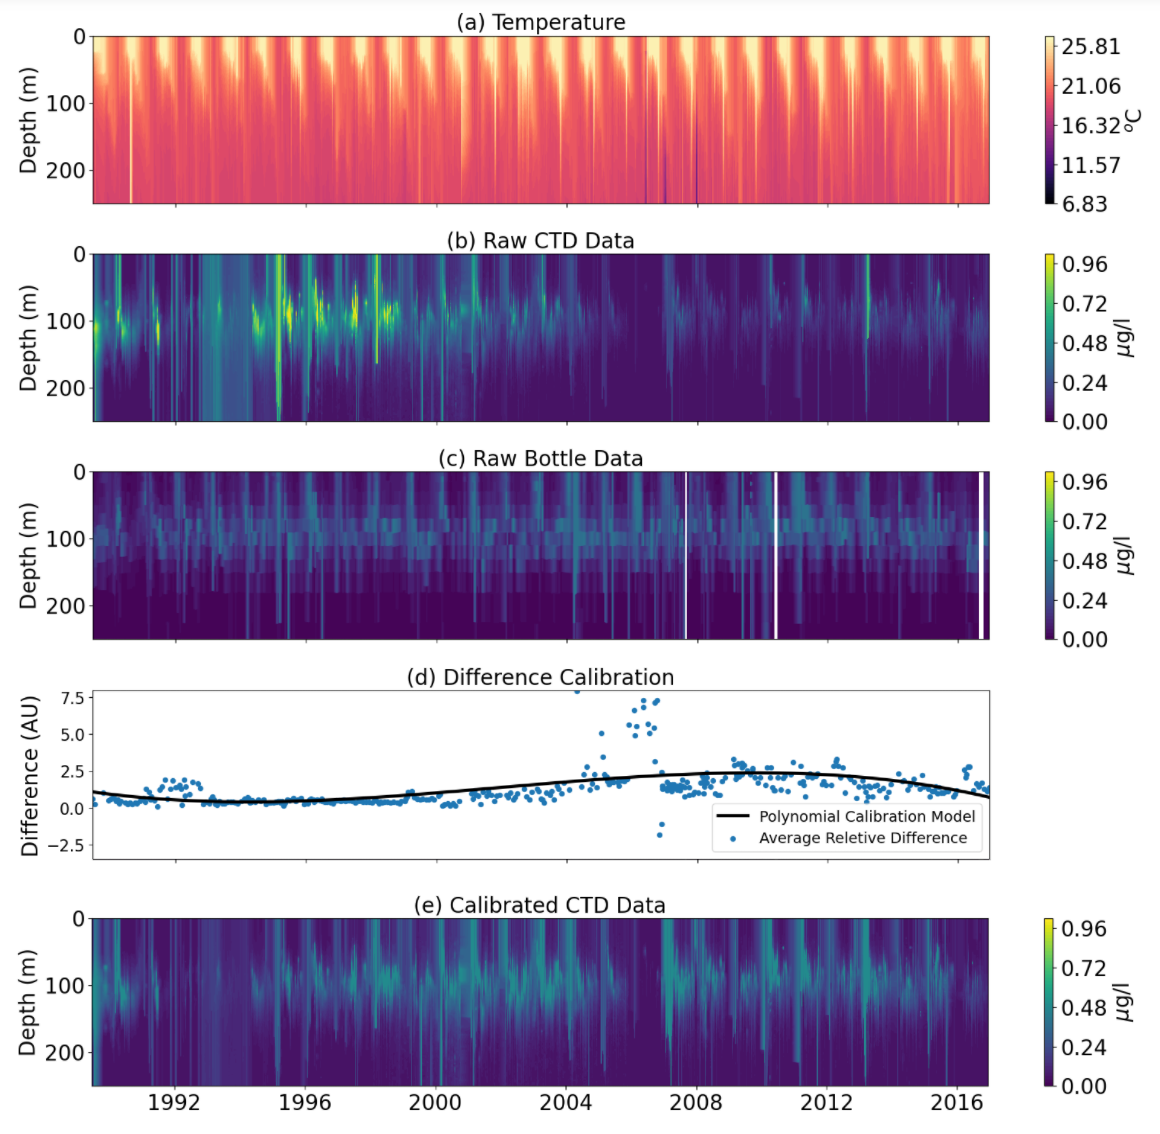
\includegraphics[height=0.945\textwidth]{model_analysis_5plot.PNG}
\end{center}
\caption{Original and crunched vertical profile data from the Bermuda Atlantic Time-series Study from June 1989 to December 2016. (a) Temperature measurements from the CTD dataset. (b) Chlorophyll-a concentration measurements from the CTD dataset. (c) Chlorophyll-a concentration combined from Turner and HPLC measurements from the Bottle data. (d) Average Relative Difference (arbitrary units (AU)) between vertical Chl-a profiles from the Bottle dataset and corresponding profiles from the CTD dataset. (e) Chlorophyll-a concentration data from the final calibrated CTD dataset that was interrogated in this study. For contour plots, data were interpolated for each plot (Python function scipy.interpolate.interp1d) extrapolating for missing values. Artefacts visible on these plots are a result of this process.}
\end{figure}
\noindent
The BATS site displayed seasonal variation in temperature readings, with cooler readings and an absence of an observable thermocline in winter periods and the presence of a warmer layer above the thermocline in summer periods (Figure 1a).\\ \\
\noindent
4653 of CTD profiles were appropriate for Mixed Layer Depth (MLD) calculation. Mean average MLD occurred at a depth of 51.8m ($Q1 = 23.7m$, $Q3 = 63.5m$). \\ \\
\noindent
The average Chl-a reading from the CTD data was 0.0602$\mu g$ $l ^{-1}$ ($Q1 = 0.0130\mu g$ $l ^{-1}$, $Q3 = 0.0550$ $\mu g$ $l ^{-1}$) (Figure 1b). The average Chl-a reading from the Bottle data was 0.0464$\mu g$ $l ^{-1}$ ($Q1 = 0.0015$$\mu g$ $l ^{-1}$, $Q3 = 0.0490$$\mu g$ $l ^{-1}$) (Figure 1c).\\ \\
\noindent
For the first $\sim$14 years of the BATS, averaged Bottle vertical Chl-a profiles were mostly lower than their corresponding CTD profiles, whereas, in the latter $\sim$14 years of the study, they were mostly higher than their corresponding CTD profiles (Figure 1d).\\ \\
\noindent
Polynomial regression was used on the difference in CTD Chl-a concentration and Bottle Chl-a concentration to create a calibration model. This calibration model, as seen in Figure 1d, demonstrates the average relative difference in vertical Chl-a profiles of the CTD and Bottle datasets. Where the model exceeds 1AU, average Chl-a profiles of the Bottle Dataset are predicted to be higher than average Chl-a profiles of the CTD Dataset. \\ \\
\noindent
The fitted regression model: \scalebox{1}{$y = -0.001061 x^{3} + 6.374 x^{2} - 12760 x + 8516000$} \\
where x is the decimal year the profiles were taken and y is the average relative difference between profiles in the dataset. The Median Absolute Error of the model was 0.4216AU (Polynomial Calibration Model, Figure 1d) \\ \\
The average relative difference of Bottle to CTD Chl-a profiles deviated for a period early on around 1992 where Bottle Chl-a profiles were mostly higher than CTD fluorescence profiles. Most outliers were found between 2004 and 2008 where the difference in Chl-a readings in Bottle and CTD profiles was much higher (Figure 1d). \\ \\
Correction and calibration of the CTD dataset resulted in a final dataset covering the water column at the BATS from June 1989 through December 2016, totalling 1624724 observations over 4653 vertical profiles (Figure 1e). The dataset contained two periods of reduced profile frequency occurring between 1992 and 1995 and in 2007 (Figure 1e). This dataset displayed a minimisation of outlier Chl-a readings when compared with the raw CTD dataset, notably between 1994 and 1998.
\subsection{Modelling of CTD Data}
% \setlength{\textwidth}{500pt}

In the top 250m of the water column, the average Chl-a concentration of the calibrated CTD data was 0.1234$\mu g$ $l ^{-1}$ ($Q1 = 0.0422\mu g$ $l ^{-1}$, $Q3 = 0.1691\mu g$ $l ^{-1}$) (Figure 2a). \\ \\
The partitioning model was successfully applied to all the profiles across the calibrated CTD dataset bar two small periods in 2007 and 2008 (Figure 2b). Average Chl-a concentration of the model was 0.1043$\mu g$ $l ^{-1}$ ($Q1 = 0.0008\mu g$ $l ^{-1}$, $Q3 = 0.1691\mu g$ $l ^{-1}$) (Figure 2b).\\ \\
The model fits well to the data with a slight propensity to underestimate Chl-a concentration. The mean average difference between the data and the model Chl-a concentration was \textminus 0.0220$\mu g$ $l ^{-1}$ ($Q1 = - 0.0412\mu g$ $l ^{-1}$, $Q3 = - 0.0001\mu g$ $l ^{-1}$). Underestimation of the Chl-a concentration by the model was more common at depths below $\sim 130$m while overestimation of the Chl-a concentration by the model was more common in between 40m and 130m (Figure 2c).\\ \\
During the study time-frame, the model surface community was most active within the upper $\sim 75$m of the water column, showing increases in the depth and intensity of Chl-a concentrations at seasonal peaks, which coincided with increases in the MLD (Figure 2d).\\ \\
The model subsurface community partition was most active between $\sim$50-175m in the water column displaying regular decreases in Chl-a concentration, which also coincided with increases in the MLD (Figure 2e).%, which also coincided with increases in the MLD (Figure 2e).
\begin{figure}[ht!]
\begin{center}
      \includegraphics[height=0.945\textwidth]{model_contour.PNG}
\end{center}
\caption{The modelled chlorophyll-a vertical profiles in time from June 1989 to December 2016 in the top 250m. (a) Chlorophyll-a concentration data that were used by the Model. (b) Model Chlorophyll-a profiles. (c) Difference between the Modelled and Data Chlorophyll-a profiles. (d) Surface phytoplankton community partition of the model profiles. (e) Subsurface phytoplankton community partition of the model profiles. Data were interpolated for each plot (Python function scipy.interpolate.interp1d) extrapolating for missing values. Artefacts visible on these plots are a result of this process. }
\end{figure}
\subsection{Integrated Chlorophyll-a Analysis}

\noindent
Least square linear regression was used to test if the integrated Chl-a concentration profiles of the (i) Complete Dataset, (ii) Complete Model, (iii) Surface Community Partition Model and (iv) Subsurface Community Partition Model significantly changed over time.
\begin{figure}[ht!]
\begin{center}
      \includegraphics[width=1\textwidth]{Analysis.PNG}
\end{center}
\caption{Trends in integrated Chlorophyll-a concentration profiles at the BATS from June 1989 to December 2016. (a) Integrated vertical profiles of Chlorophyll-a concentration of the processed data and complete model. (b) Integrated vertical profiles of Chlorophyll-a concentration of the surface phytoplankton community partition model. (c) Integrated vertical profiles of Chlorophyll-a concentration of the subsurface phytoplankton community partition model. Profile integrations were conducted down to 1.5x the euphotic depth ($Z_p$).}
\end{figure}
\begin{enumerate}[(i)]
    \item Least square linear regression indicates that, when using the final dataset, total profile Chl-a over the BATS shows no significant change with time (\textit{R}$^2$ < 0.001, \textit{t}$_{4653}$ = 175.156, \textit{P} = 0.173; y = 54.621 - 0.018x; Figure 3a).
    \item Least square linear regression indicates that, when using the model, total profile Chl-a over the BATS shows no significant trend with time (\textit{R}$^2$ < 0.001, \textit{t}$_{4653}$ = 170.880, \textit{P} = 0.532; y = 0.009x + 0.451; Figure 3a).
    \item Least square linear regression indicates that total profile Chl-a of the surface community over the BATS decreases significantly with time (\textit{R}$^2$ = 0.026, \textit{t}$_{4653}$ = 76.143, \textit{P} < 0.001; y = 260.554 - 0.127x; Figure 3b). 
    \item Least square linear regression indicates that total profile Chl-a of the subsurface community over the BATS increases significantly with time (\textit{R}$^2$ = 0.014, \textit{t}$_{4653}$ = 83.960, \textit{P} < 0.001; y = 0.135x - 260.103; Figure 3c). 
\end{enumerate}

\section{Discussion}
The data collected by the Bermuda Atlantic Time-series Study provided the opportunity to study vertical changes in phytoplankton biomass in the water column of a single location across 28 years. In this report, a phytoplankton community partitioning model has been applied to BATS Chl-a data for the first time. In achieving this study's aim, it is shown that the total Chl-a in the subsurface phytoplankton community has increased significantly over this time while the total Chl-a in the surface phytoplankton community has decreased. However, there was no significant change in the total Chl-a of phytoplankton. These trends suggest that over the BATS the biomass of phytoplankton in the subsurface community increased while the surface community decreased. 
\subsection{Seasonality}
Superficial investigations into the seasonality of the data revealed expected similarities between the BATS site and other subtropical oligotrophic waters. Temperature profiles from the BATS displayed seasonal variation in the upper depths of the water column, with warmer readings occurring at increasingly deeper depths into the summer months as the thermocline deepened throughout the season, transitioning to cooler readings as the water column completely mixed around the winter months. MLDs of profiles also indicated seasonality, increasing over summer months, before peaking and then sharply declining to the annual low ($\sim$20m) around January every year. This seasonal pattern of temperature is comparable to other subtropical oligotrophic waters like those at the Gulf of Naples and the North Pacific Ocean \citep{peralba_vertical_2004,dore_seasonal_2002}. The location of the BATS was selected based on this similarity to other subtropical gyre regions \citep{alkire_using_2013}, giving weak evidence that the results of this study are important to many other ocean regions \citep{morel_most_2010}.
\subsection{Difference Calibration}
The average relative difference between the Bottle and CTD profiles displayed change over time. These changes can likely be attributed to the recalibration and swapping of the fluorometers used by the survey vessels over the course of the study \citep{johnson_chapter_nodate-1}. \\ \\
The polynomial calibration model represented the average relative difference between the datasets with varying degrees of success. Small overall changes in difference were well modelled; however, larger variation between CTD and Bottle profiles around 1992 and after 2004 were not well represented by the model. \\ \\
After correction and calibration, the CTD dataset was more consistent with the Bottle data. However, inconsistencies remained; where the Bottle data displayed near-zero readings, the corresponding CTD readings were higher (Figures 1c \& 1e). 
\subsection{Model Calibration}
The model fit well to the CTD data, though when compared it underestimated Chl-a below $\sim$150m (Figure 2c). This lowering of near-zero readings increased their similarity to the more accurate Bottle Chl-a readings, seemingly making the model more accurate than the CTD data (Figures 1c \& 2b).
\subsection{Total community}
Contrary to a previous analysis of the BATS data, this study found no significant trend in total integrated Chl-a. Previous analysis using the BATS data from 1989-2006 concluded that total integrated Chl-a at the BATS site displayed an increasing trend in the Bottle HPLC data and a decreasing trend in the CTD fluorescence data \citep{saba_challenges_2010}. Inconsistencies between these results and those from this study may be explained by the recent additions to the dataset from 2006-2016. An additional explanation may be the different methods of data analysis used in our studies, as the CTD data were not corrected and calibrated in their study. \\ \\
Using Chl-a as a proxy for biomass \citep{boyce_global_2010}, the lack of a significant trend in total Chl-a indicates that phytoplankton biomass at the BATS site is not changing. This implies that at the BATS site, phytoplankton biomass is relatively resistant to the rising sea temperatures observed at all depths in the region \citep{joyce_long-term_1996,bonhommeau_fluctuations_2008}.
\subsection{Surface community}
The trend of decreasing Chl-a in the surface phytoplankton community model aligns consistently with current research. In most of the world’s oceans, surface phytoplankton also show long-term declines \citep{boyce_global_2010}. As changes in biomass are indicative of shifts in phytoplankton community composition \citep{mcquatters-gollop_long-term_2007}, this decrease in Chl-a is expected as temperature-induced changes in species composition have been found in the surface phytoplankton community in the Sargasso Sea \citep{lomas_adaptive_2022}. This community’s decline may indicate that as in many other ocean regions, the surface phytoplankton community biomass at the BATS site is declining due to the rising sea surface temperatures (SSTs) in the region \citep{boyce_global_2010,liu_variability_2019,sheppard_sea_2005}. As continued rises in SST are projected due to anthropogenic climate forcing \citep{sheppard_sea_2005,alexander_projected_2018}, the surface phytoplankton community biomass may continue to decline at the BATS site. \\ \\
This community’s primary production has been found to mirror its decline in biomass \citep{lomas_adaptive_2022}, signposting how climate change may be altering its role in nutrient cycling and ecosystem function \citep{mcmahon_millennial-scale_2015,winder_phytoplankton_2012}. However, a recent study from \citep{lomas_adaptive_2022} observed temperature-induced community changes in the BATS surface community that maintained its levels of carbon export. This suggests the potential of phytoplankton communities to adapt to environmental changes through changes in species composition, preventing consequential changes to certain biogeochemical cycles despite declines in biomass.
\subsection{Subsurface community}
Integrated Chl-a of the subsurface community displayed a significant increasing trend. This suggests that the biomass of the subsurface phytoplankton community at the BATS site is also increasing. Implying that while the surface community biomass is falling, total phytoplankton biomass is not in decline due to an opposing rise in subsurface phytoplankton. These shifts may arise from each community being affected disproportionately by climate forcing impacts such as rising SSTs \citep{liu_variability_2019,sheppard_sea_2005}. Whereby increased stratification of the water column caused by rising SSTs may be lowering phytoplankton growth rates in the surface community by reducing nutrient flux from deeper waters \citep{boyce_dg_patterns_2015,schmittner_decline_2005}. The combination of less biomass and nutrients above the subsurface community could improve the water transparency to a degree that enhances light levels \citep{mcgillicuddy_covariation_2001}, this would allow for greater growth rates in this light-limited community \citep{cullen_subsurface_2015}. These results show that in subtropical ocean gyre regions, despite declining trends in surface phytoplankton, total phytoplankton biomass might not be declining. If so, further study of the simultaneous changes in species composition and vertical distribution that could be causing these trends could alter current predictions of global biogeochemical cycle changes \citep{mcmahon_millennial-scale_2015,boyce_global_2010,falkowski_role_1994,lomas_adaptive_2022}.
\subsection{Limitations and Recommendations}
It is important to note the potential shortcomings of this study that may challenge the validity of its conclusions. Using Chl-a as a proxy for phytoplankton biomass at varying depths is less than ideal due to light attenuation affecting photoacclimation \citep{behrenfeld_beam_2006,geider_dynamic_1996,fennel_subsurface_2003}. Though Chl-a has been deemed appropriate as a proxy for biomass \citep{boyce_global_2010}, the calculation of ‘Tchl-a’ (the sum of chlorophyll-a and divinyl chlorophyll) \citep{huot_does_2007} or of a phytoplankton index \citep{ni_longphuirt_decoupling_2019} would be more appropriate in future studies. \\ \\
In this study, it would have been appropriate to utilise the Bottle dataset readings in the final dataset, especially in reference to the irregular periods in the CTD data between 1992 and 1995 and in 2007. Furthermore, the accuracy of the final dataset would likely have also benefited from a more appropriate calibration curve fitting technique such as a Lowess smoothing model \citep{seabold_statsmodels_2010}, to better account for the irregularities in the difference time-series caused by fluorometer adjustments (Figure 1d). \\ \\
The data here did not account for the effect of the North Atlantic oscillation, a phenomenon that has a large impact on climate and by extension phytoplankton biomass changes in the Sargasso Sea \citep{casey_changes_2013}. Though the large timescale of this dataset minimised the effect of climate indices, if corrected for, the resulting trends would be more accurate.\\ \\
Future research and monitoring projects regarding subsurface phytoplankton communities around the world and how they are changing are urgently needed. This is because the understanding of these communities has implications to not only marine biogeochemical cycles but by extension, to how the climate will change in response to changes in these cycles \citep{ross_blooms_2017,yasunaka_global_2022,friedlingstein_positive_2001}. One study site with available data suitable for subsurface phytoplankton modelling, as carried out in this study, is the Hawaiian Ocean Time-series.
\section{Conclusion}
This study concludes that at the BATS site, surface community phytoplankton biomass is in decline and the subsurface community is growing, thus maintaining total phytoplankton biomass. These results may indicate how phytoplankton communities in the world’s subtropical ocean gyres are adapting more rapidly than expected to the effects of anthropogenic climate forcing, through structural changes such as species composition \citep{lomas_adaptive_2022}, resulting in shifts to larger subsurface and smaller surface communities. If this is the case, these results add to the body of evidence questioning assertions of severe global phytoplankton decline, and asks the question of how marine ecosystems and nutrient cycles will be affected if climate change results in expanded subsurface phytoplankton communities \citep{mcmahon_millennial-scale_2015,boyce_global_2010,falkowski_role_1994,mcquatters-gollop_is_2011}.
\section{Acknowledgements}
I would like to take the time to thank R. Parsons, N. Nelson, the BATS scientific team and officers and crew of the RV Weatherbird II for their efforts in collecting and processing samples, and B. Brewin for the provision of the Chl-a partitioning model as well as for his guidance and support.
\addcontentsline{toc}{section}{References}
\small
%\bibliographystyle{unsrt}
% \bibliographystyle{unsrtnat}
\bibliographystyle{agsm}
\bibliography{Diss_refs.bib}

% \printbibliography
\end{document}
